\section{Data Processing Overview} \label{sec:processing}

The calibration and instrument signature removal (ISR) pipeline removes instrumental effects from science data.
For each effect observed in LSSTCam, the Rubin Science Pipelines define a calibration-generation task that produces the corresponding data product, and a correction task that applies that product during ISR.

\subsection{Detector Model} \label{sec:processing:detector-physics}
Calibration and ISR tasks are organized as a pipeline based on our current model of the detector physics.
The calibration production tasks are run in chronological order with respect to the photon transfer and data-acquisition chain, and ISR correction tasks are applied in the opposite order to the sequence in which effects accumulate along the signal path.

The algorithms and processing steps required for LSSTCam calibration and ISR were developed from measurements and analysis during electro-optical testing on the laboratory test stand at SLAC National Accelerator Laboratory, at the summit, and on the telescope in-dome during commissioning.
\citet{roodman2024lsst-9d4} gives a detailed account of system characterization work and results from these campaigns.
Figure~\ref{fig:detector-boxes} summarizes the instrumental effects identified in the photon transfer chain and their order.

\begin{figure*}[t]
    \centering
    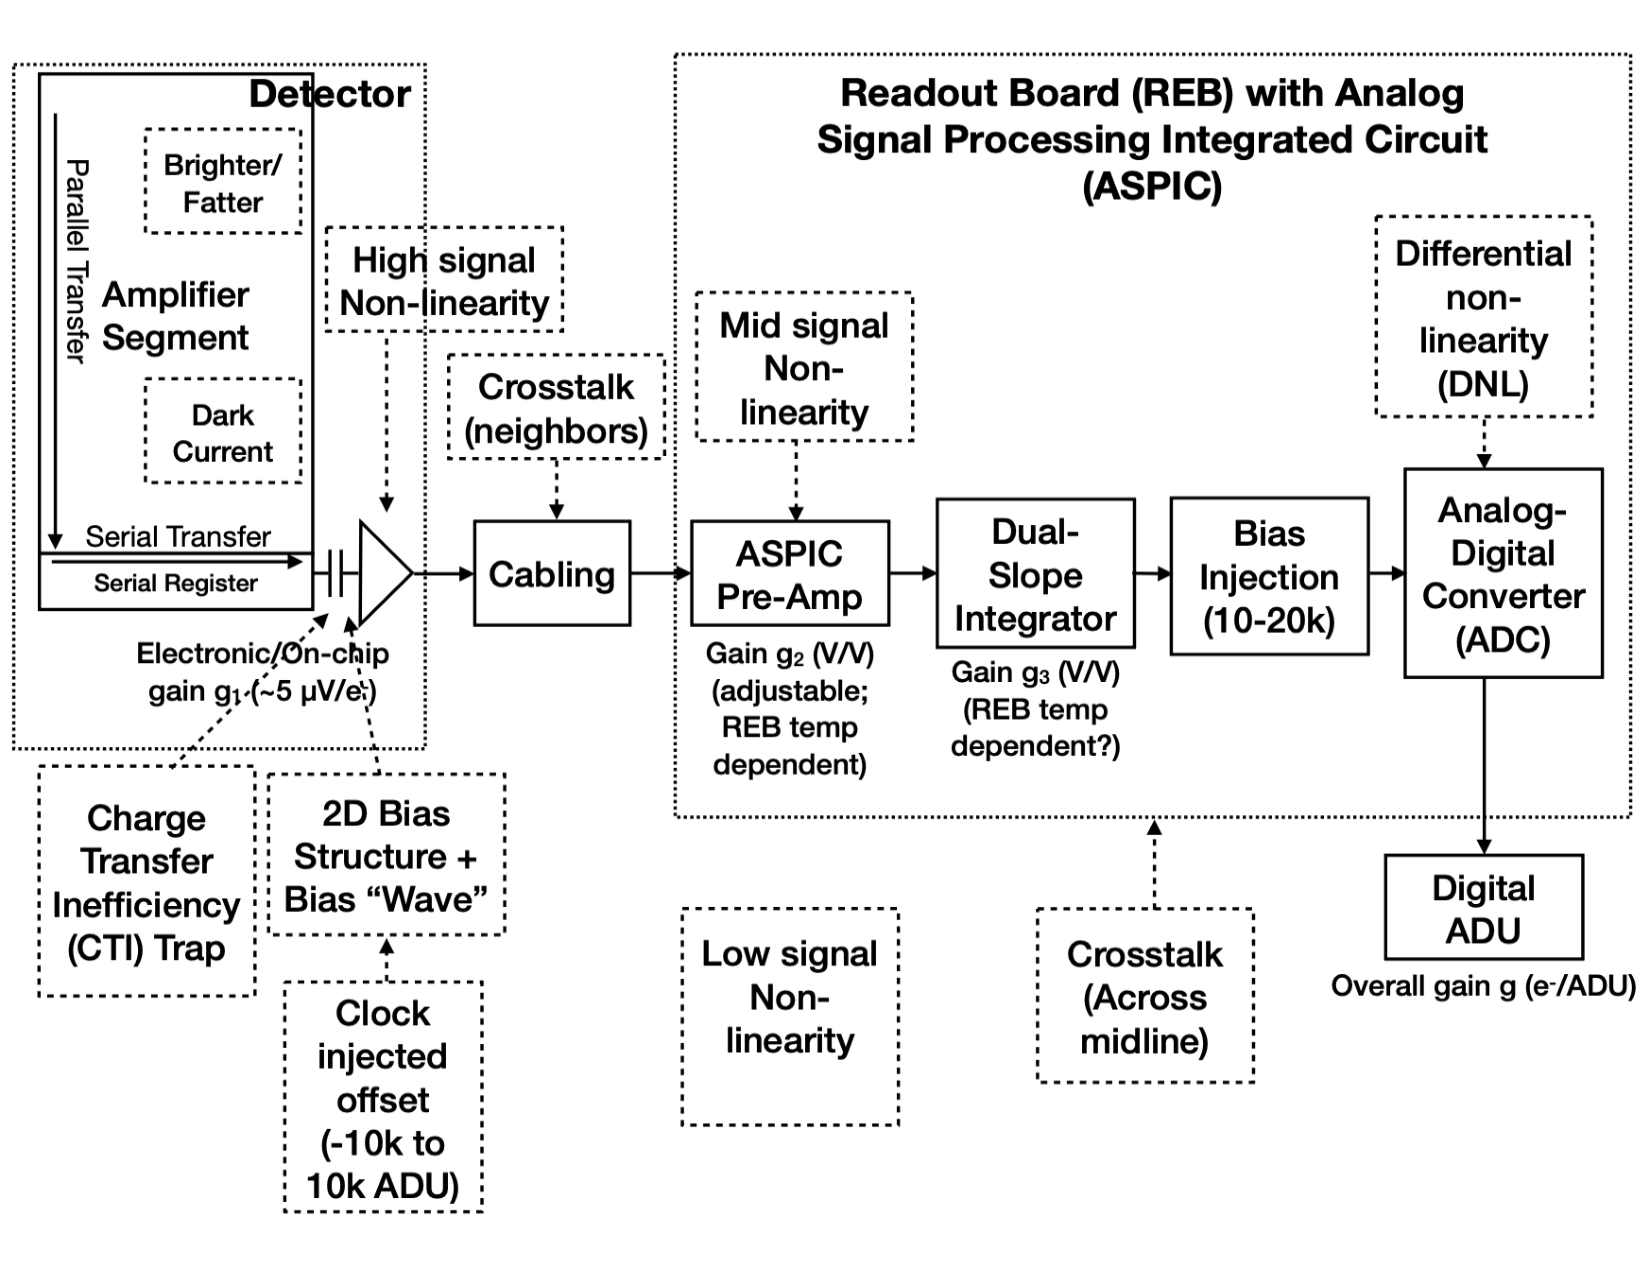
\includegraphics[width=0.8\textwidth]{figures/calibration_boxes_detector_model.pdf}
    \caption{Photon transfer and data-acquisition model for the LSSTCam detectors and electronic readout board (REB).
    Instrumental effects seen in images are shown as dashed boxes; arrows indicate where each effect enters the chain.
    Low-signal nonlinearities in LSSTCam's detector response have been observed, but their origin is not yet established; that contribution appears as a disconnected box.}
    \label{fig:detector-boxes}
\end{figure*}

... describe the detector physics ...
